\documentclass{article}
\usepackage[utf8]{inputenc}

 \usepackage{amsmath}
 \usepackage{amssymb}
 \usepackage{caption}
 \usepackage{graphicx}
 \usepackage{graphics} 
 \usepackage{textcomp}
 \usepackage{epsfig} 			
 \usepackage{mathptmx} 			
 \usepackage{times}

 \usepackage{dsfont}
 \usepackage{epsfig}
 \usepackage{ stmaryrd}



\begin{document}

\begin{figure}
    \centering
    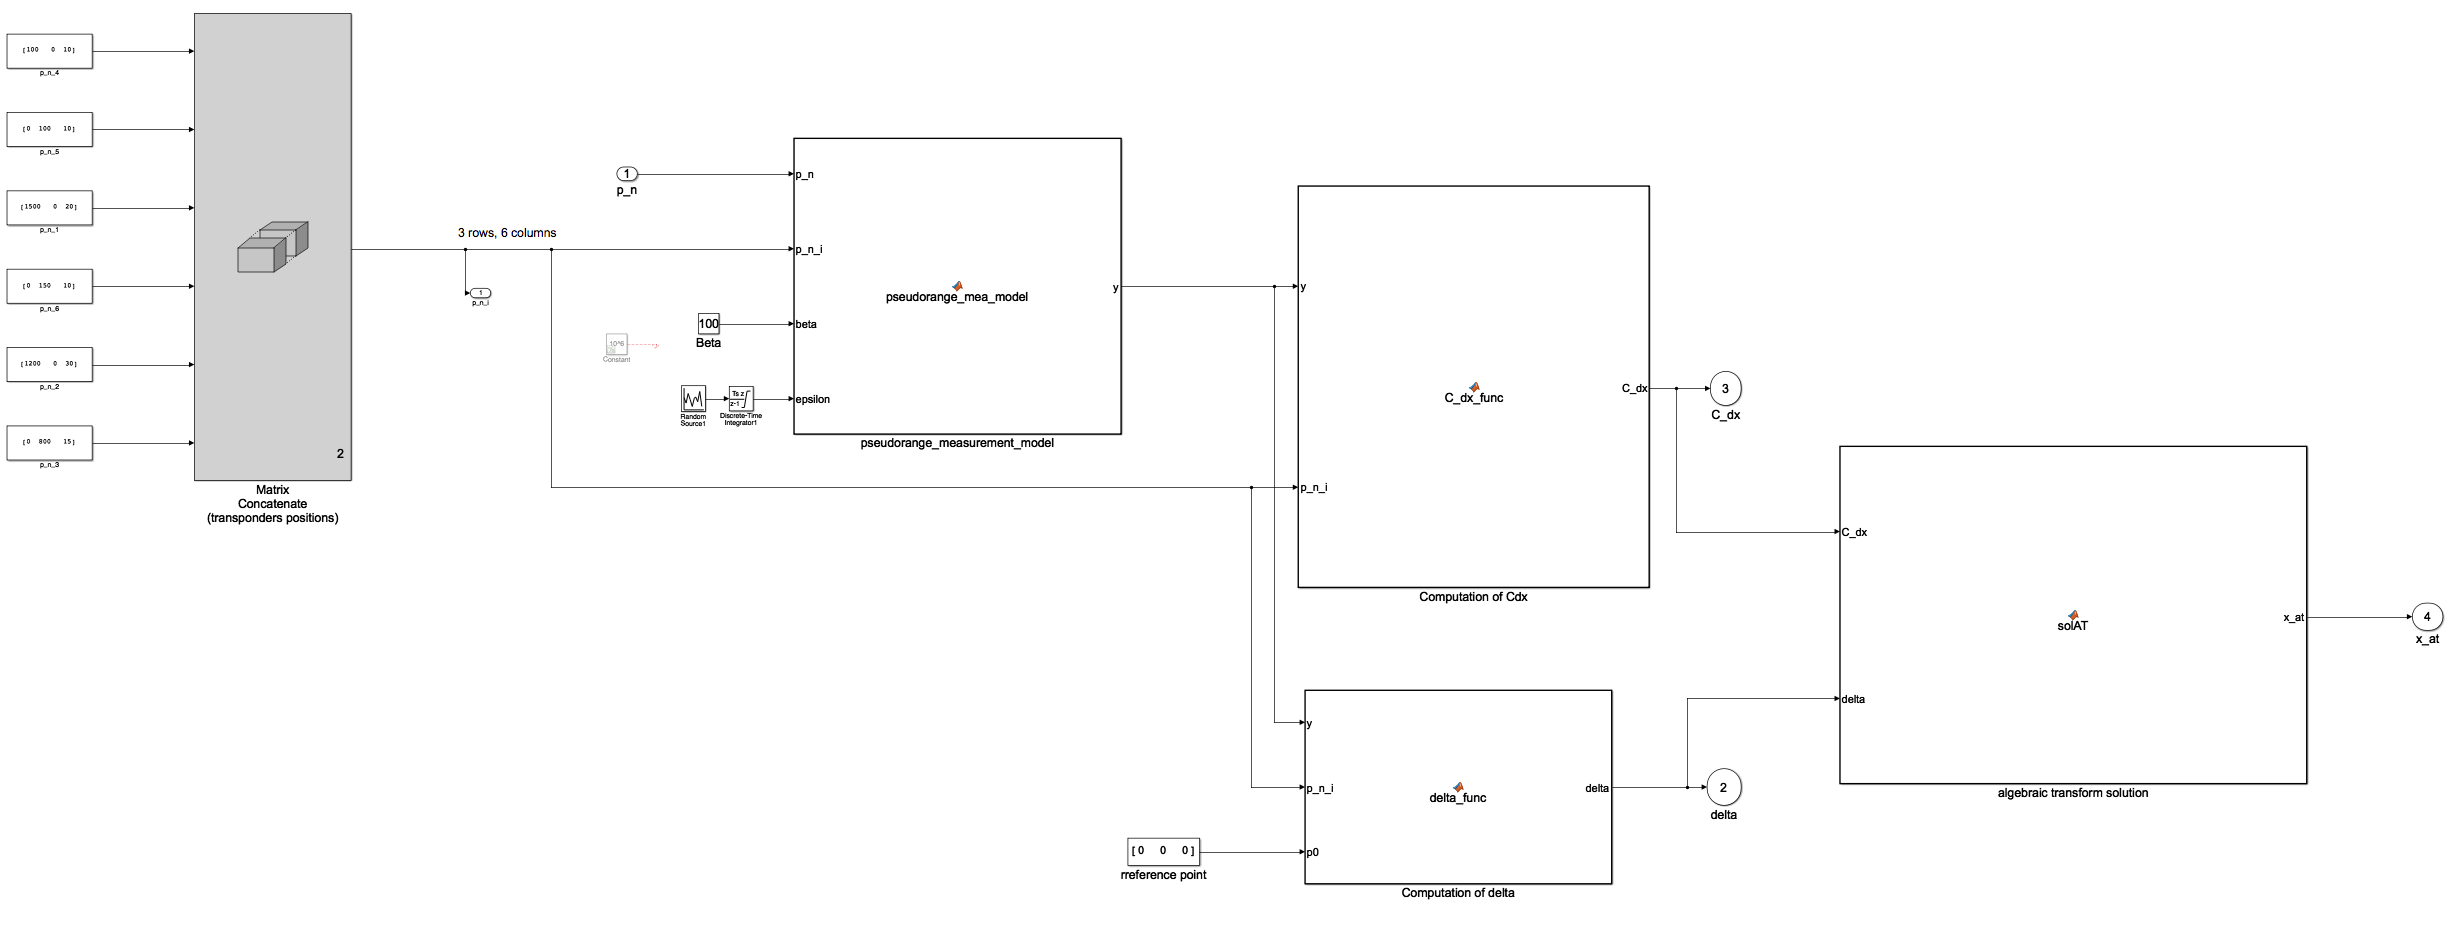
\includegraphics[angle=90,scale = 0.5]{algebraic_transf_scheme.png}
    \caption{Algebric transformation block.}
    \label{fig:f1}
\end{figure}

\begin{figure}
    \centering
    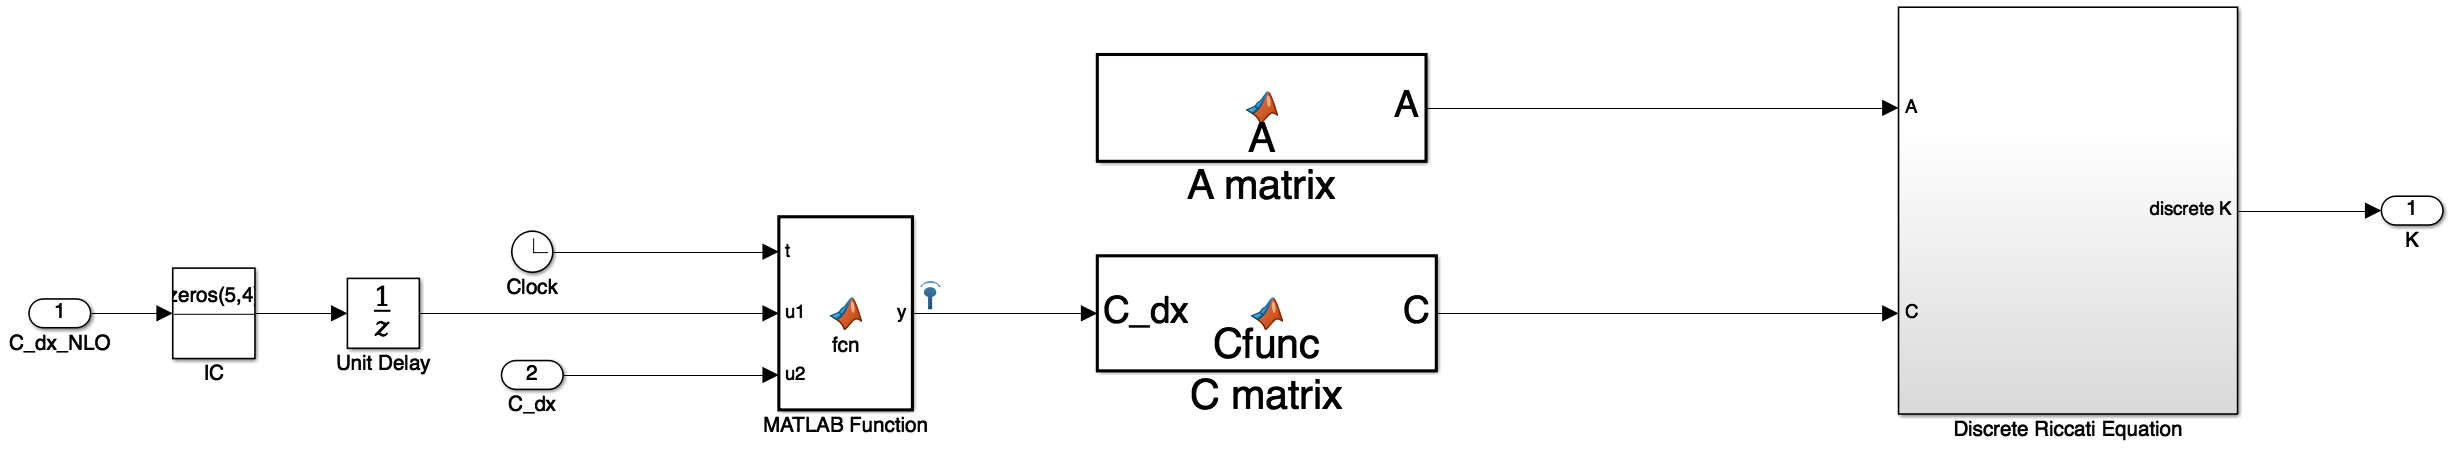
\includegraphics[angle=90,scale = 0.5]{gain_scheme.png}
    \caption{Gain computation block.}
    \label{fig:f2}
\end{figure}

\begin{figure}
    \centering
    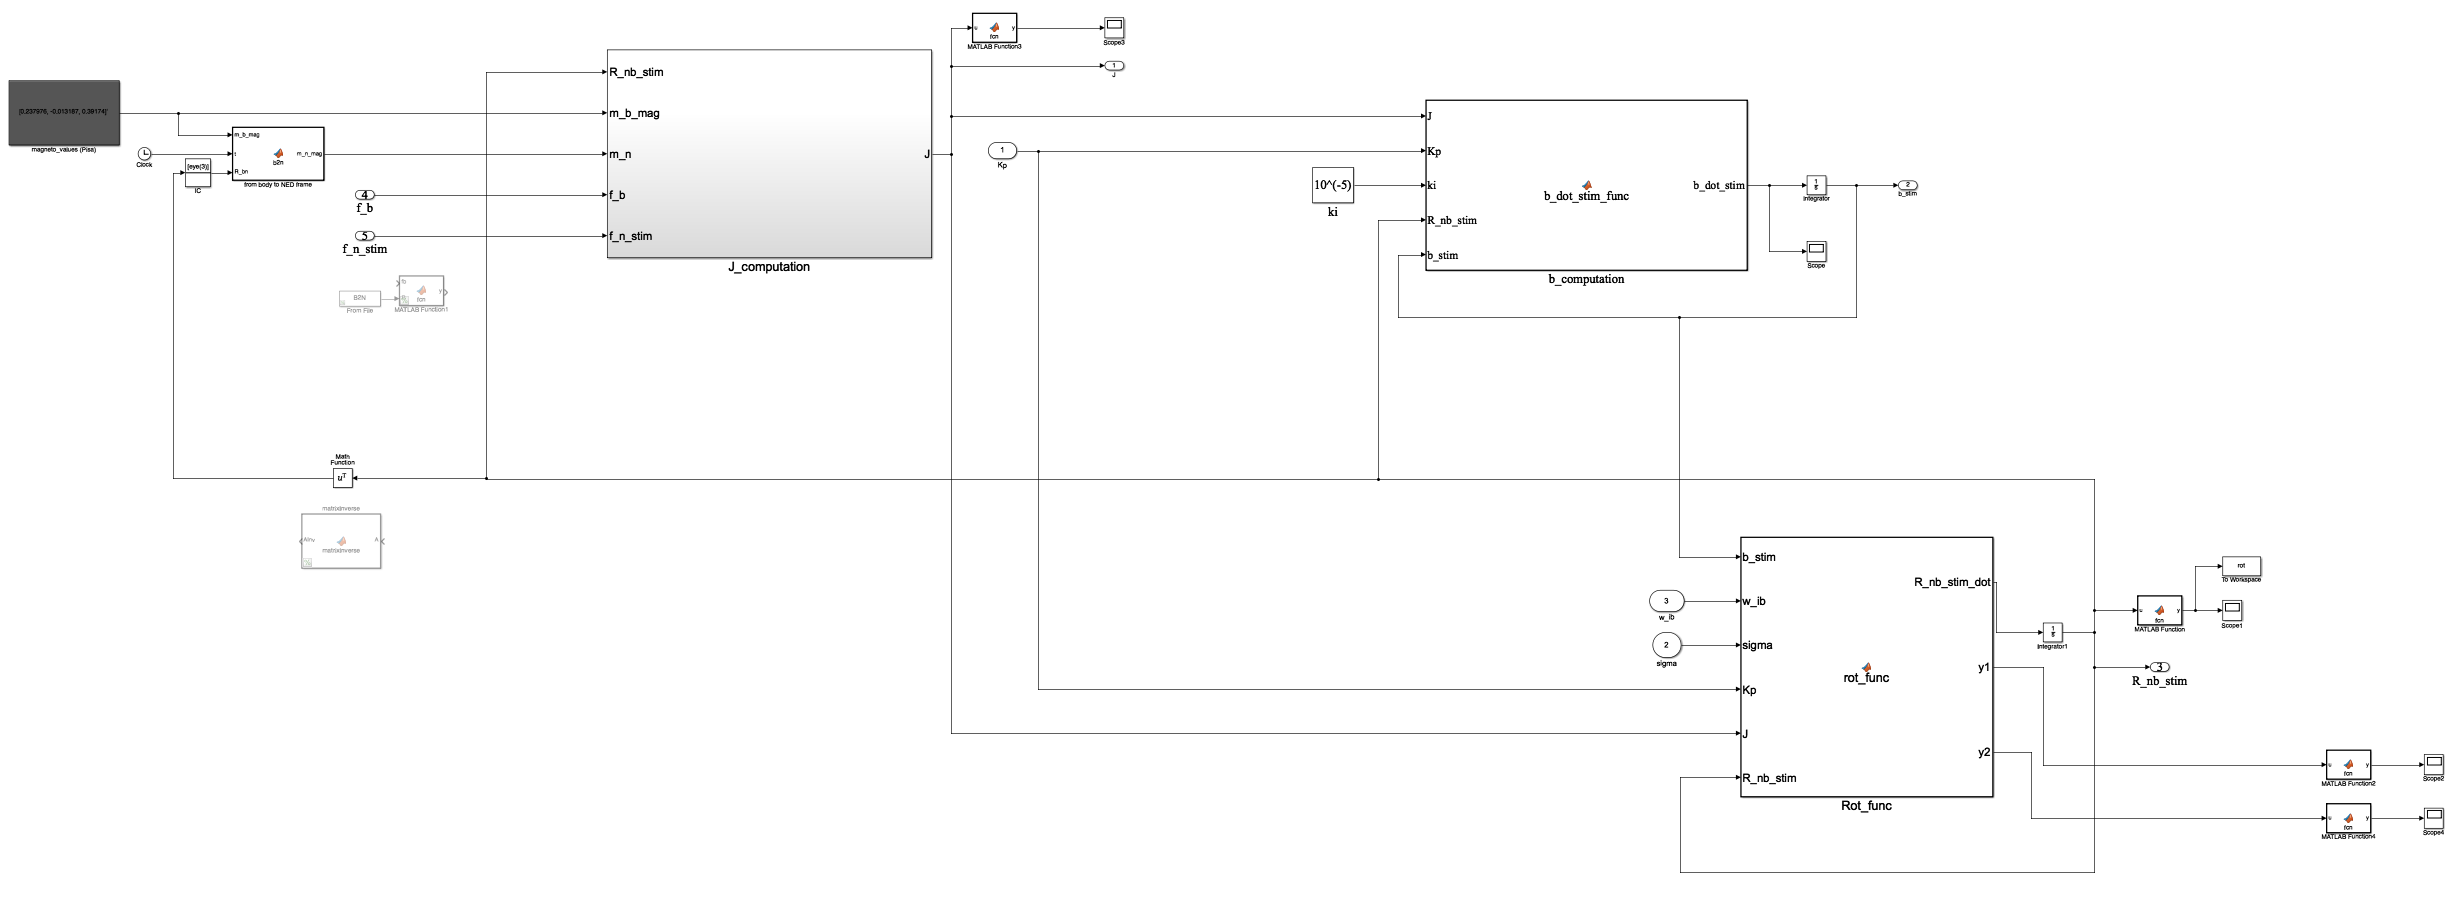
\includegraphics[angle=90,scale = 0.5]{attitude_observer_scheme.png}
    \caption{AO block.}
    \label{fig:f3}
\end{figure}


\begin{figure}
    \centering
    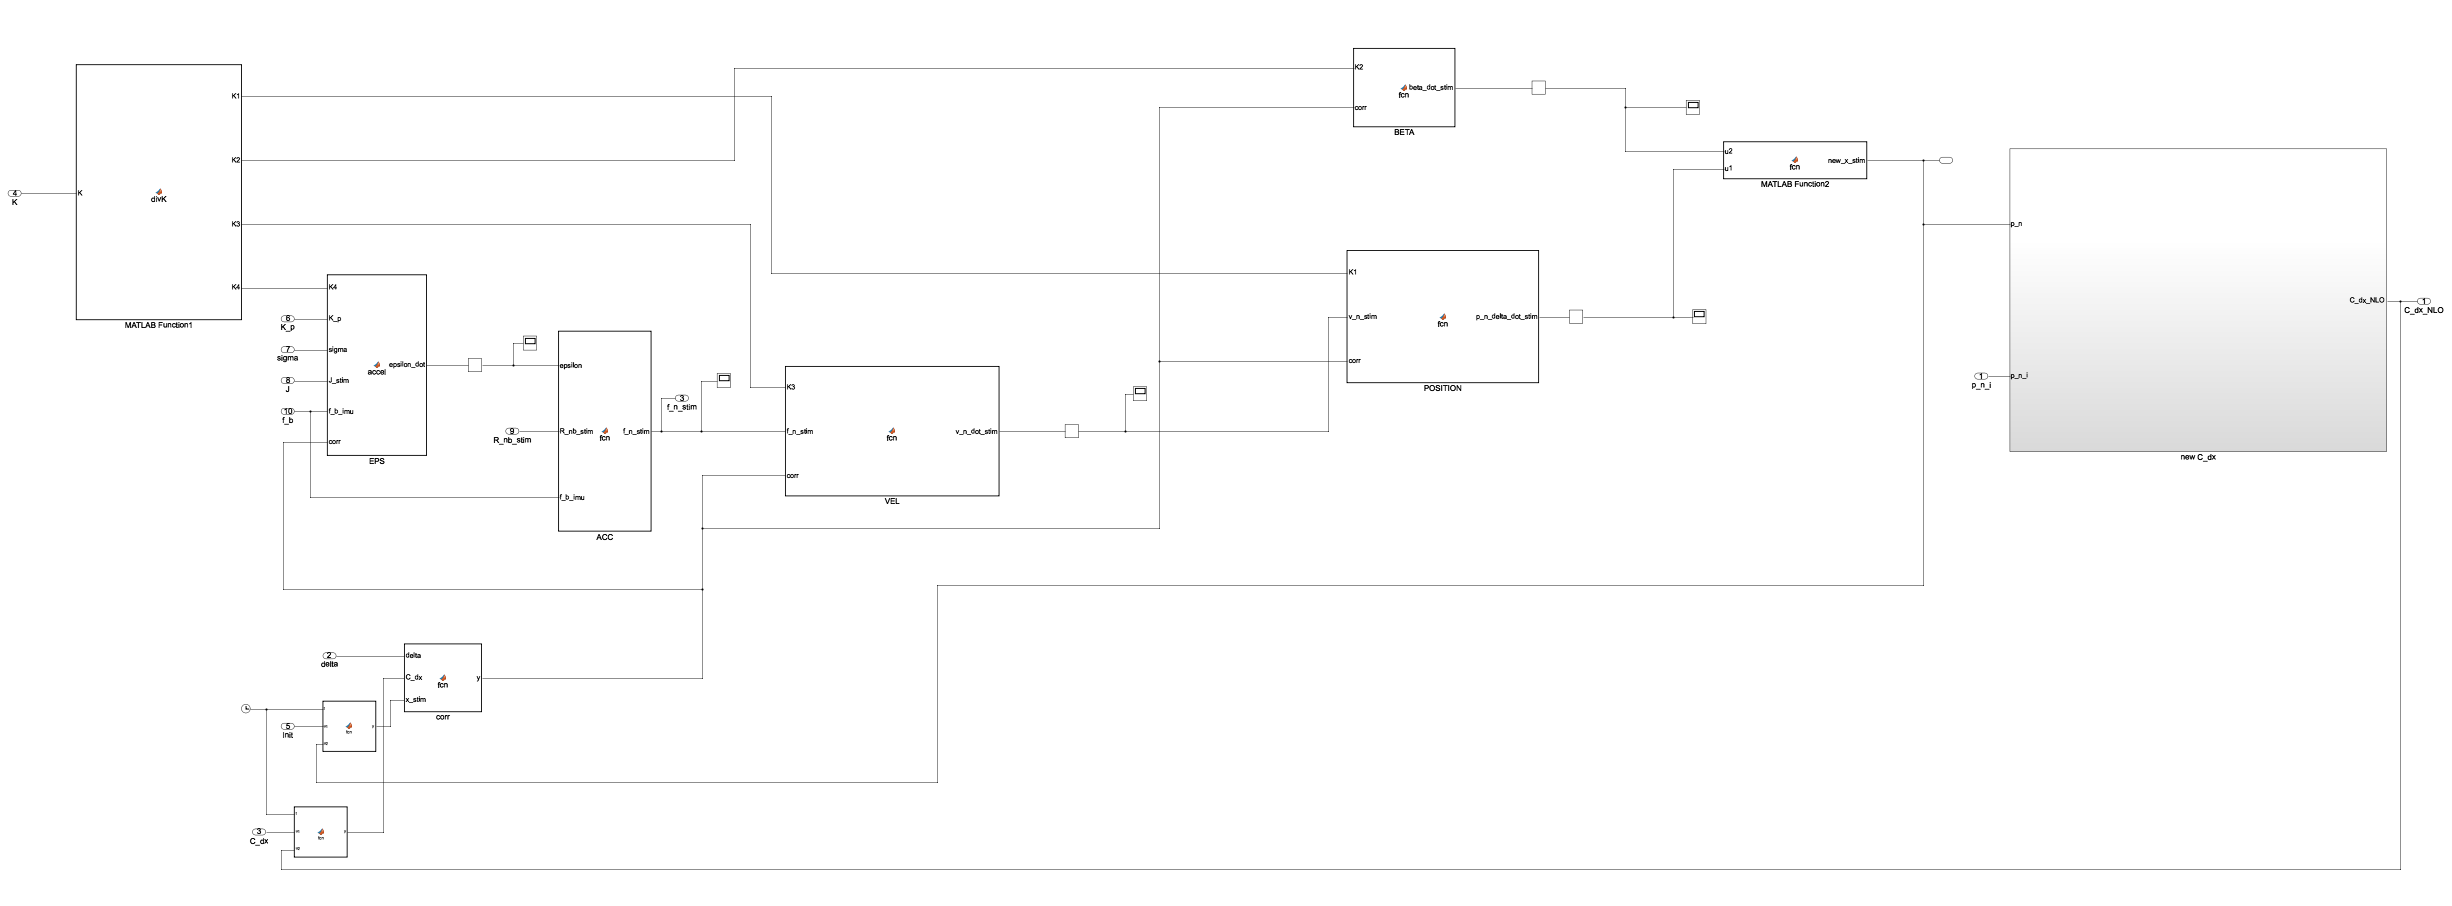
\includegraphics[angle=90,scale = 0.5]{TMO_scheme.png}
    \caption{TMO block.}
    \label{fig:f4}
\end{figure}



\begin{figure}
    \centering
    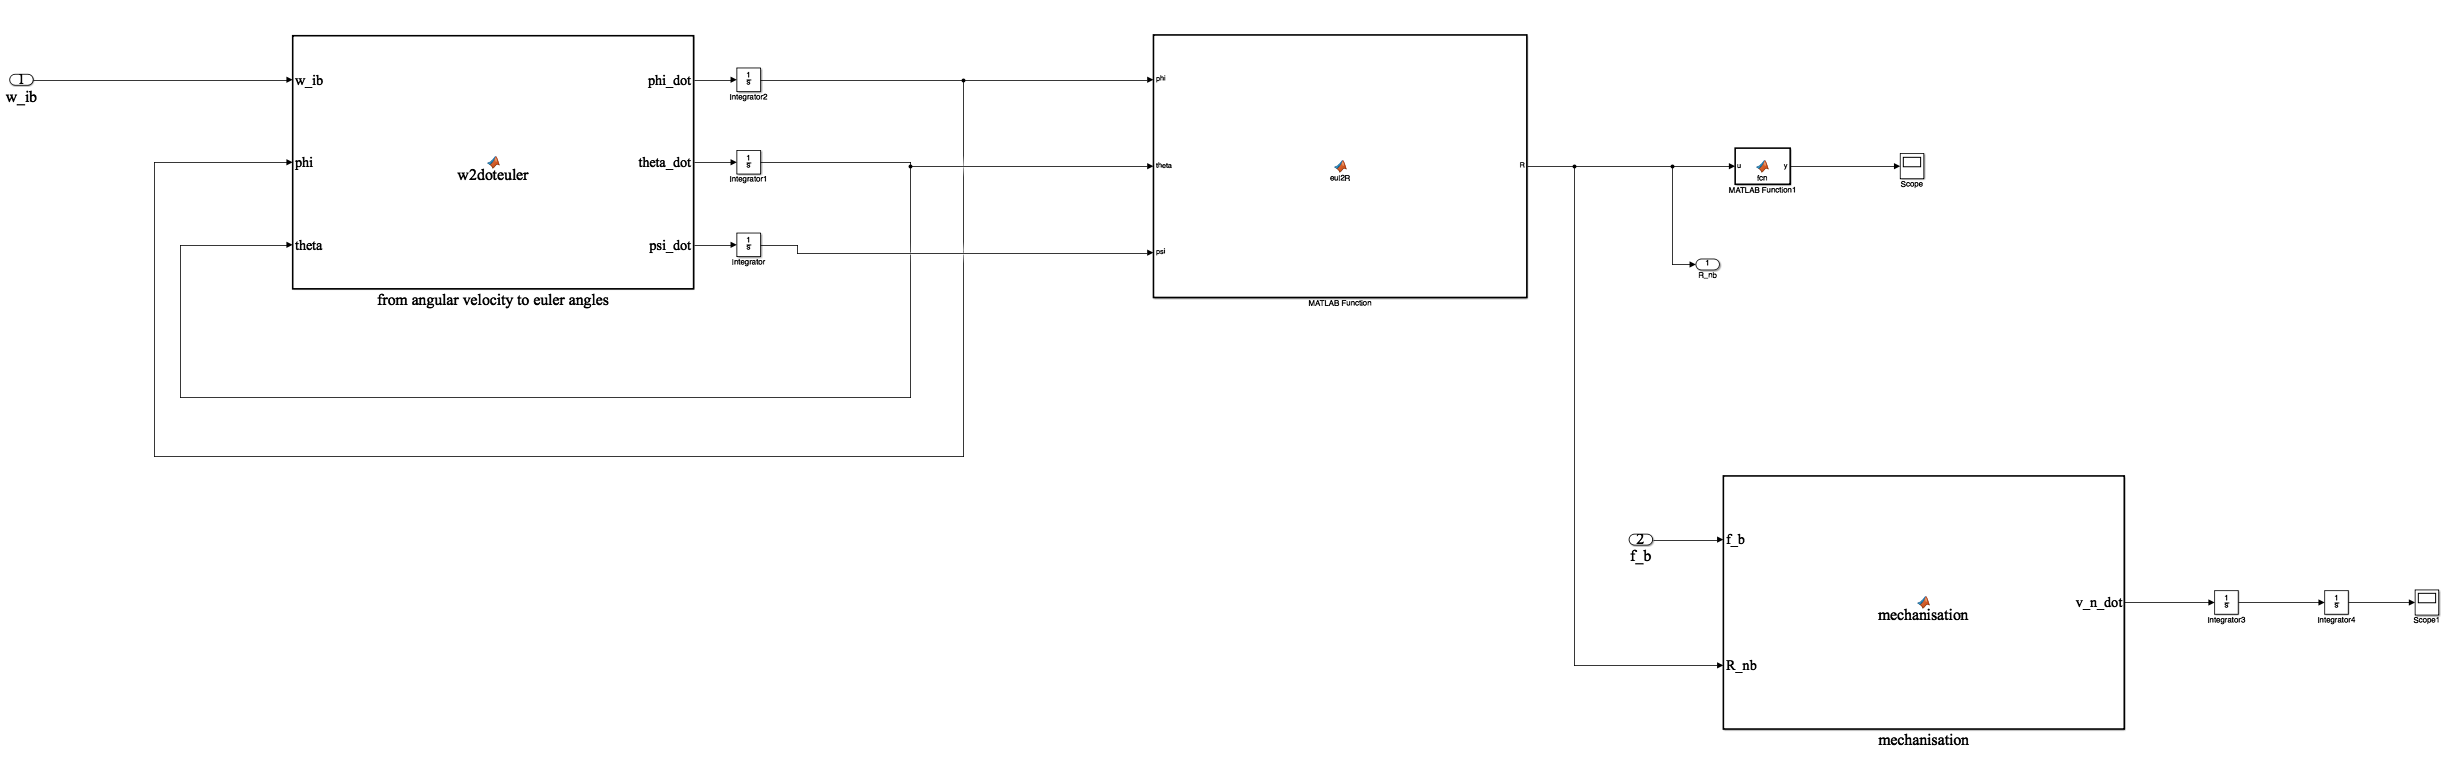
\includegraphics[angle=90,scale = 0.5]{mechanization_scheme.png}
    \caption{Mechanization block.}
    \label{fig:f5}
\end{figure}



\begin{figure}
    \centering
    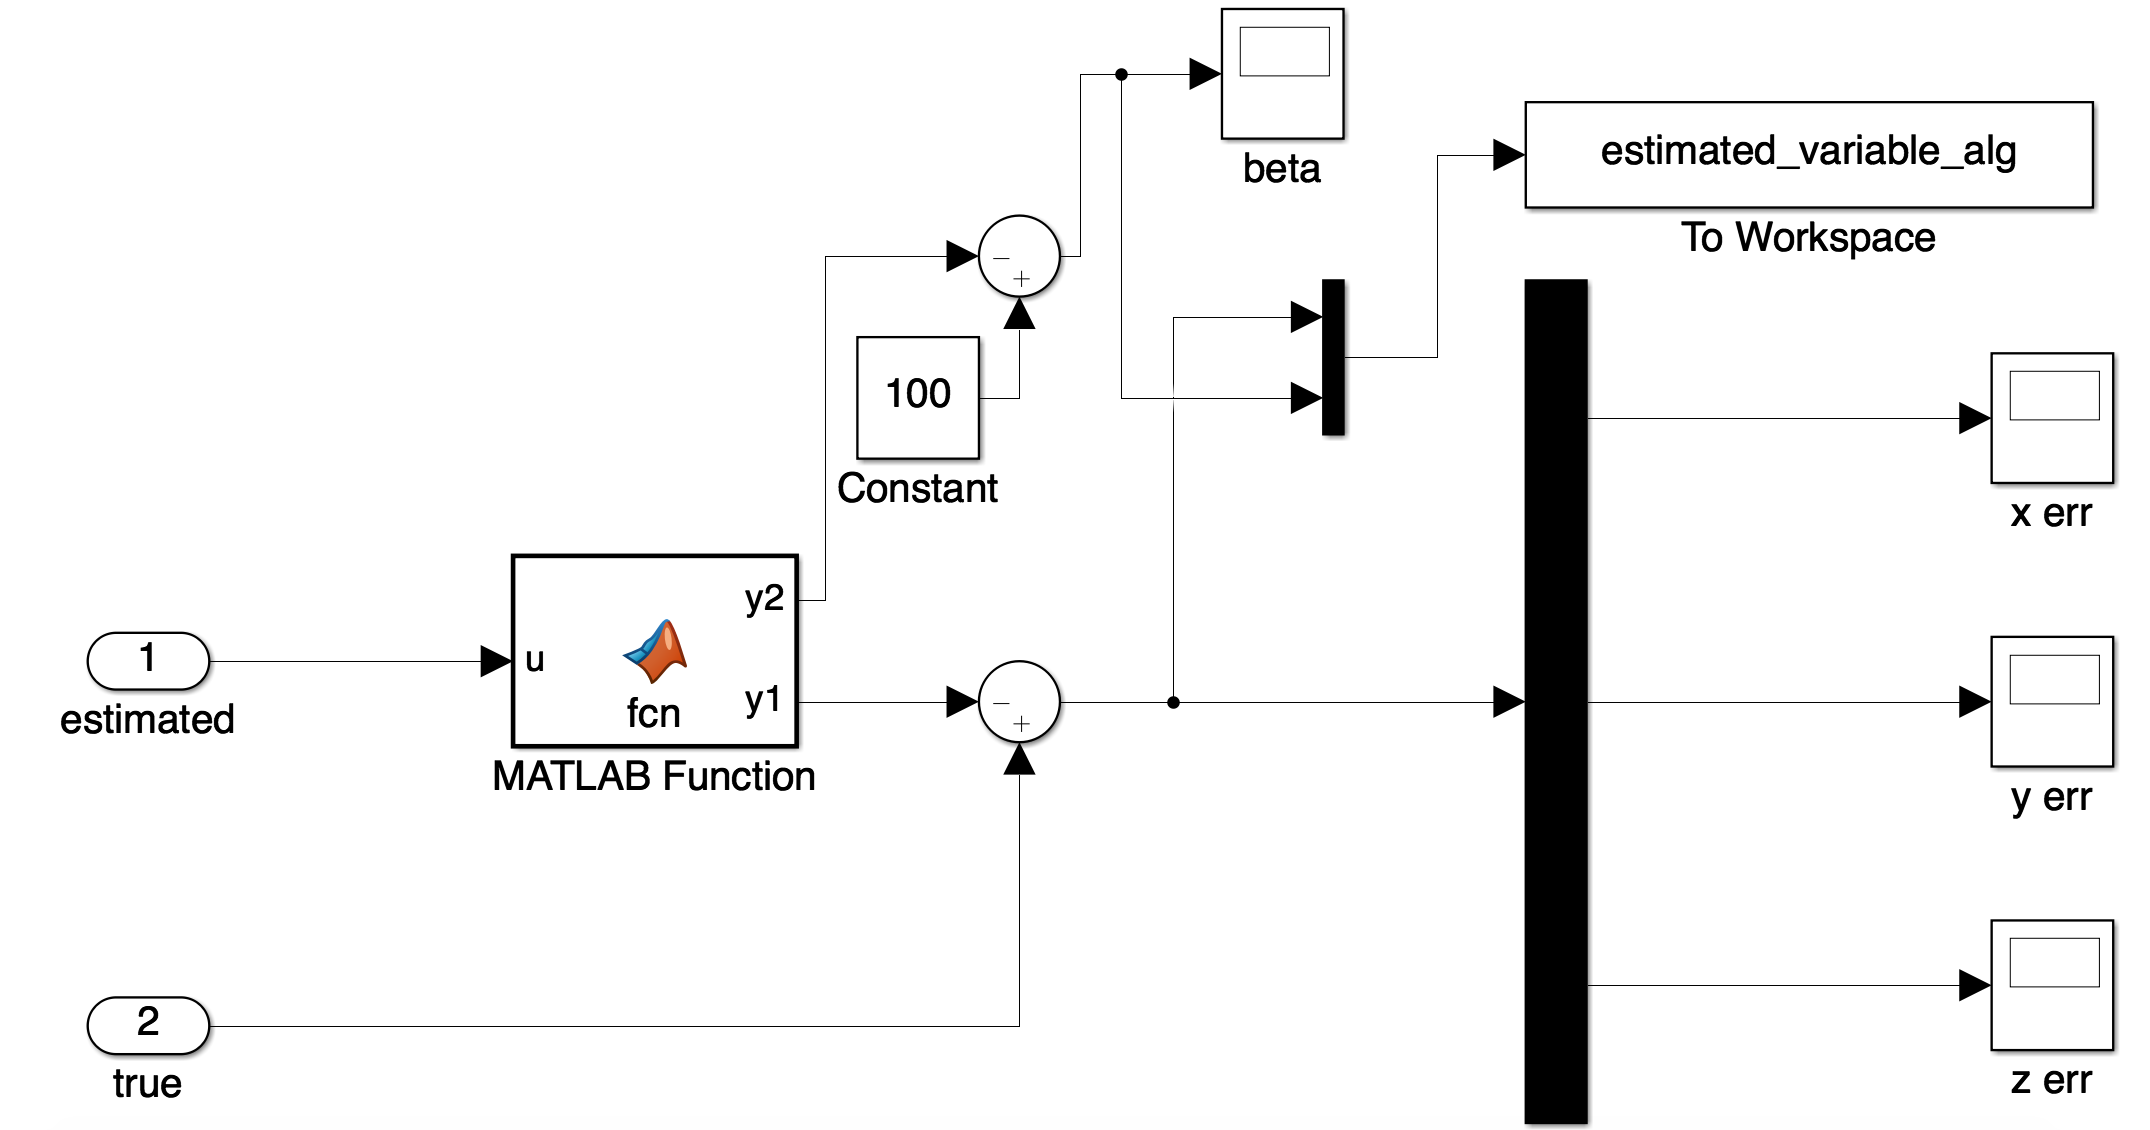
\includegraphics[angle=90,scale = 0.5]{plot_error_algebraic.png}
    \caption{Error algebraic plots block.}
    \label{fig:f6}
\end{figure}

\begin{figure}
    \centering
    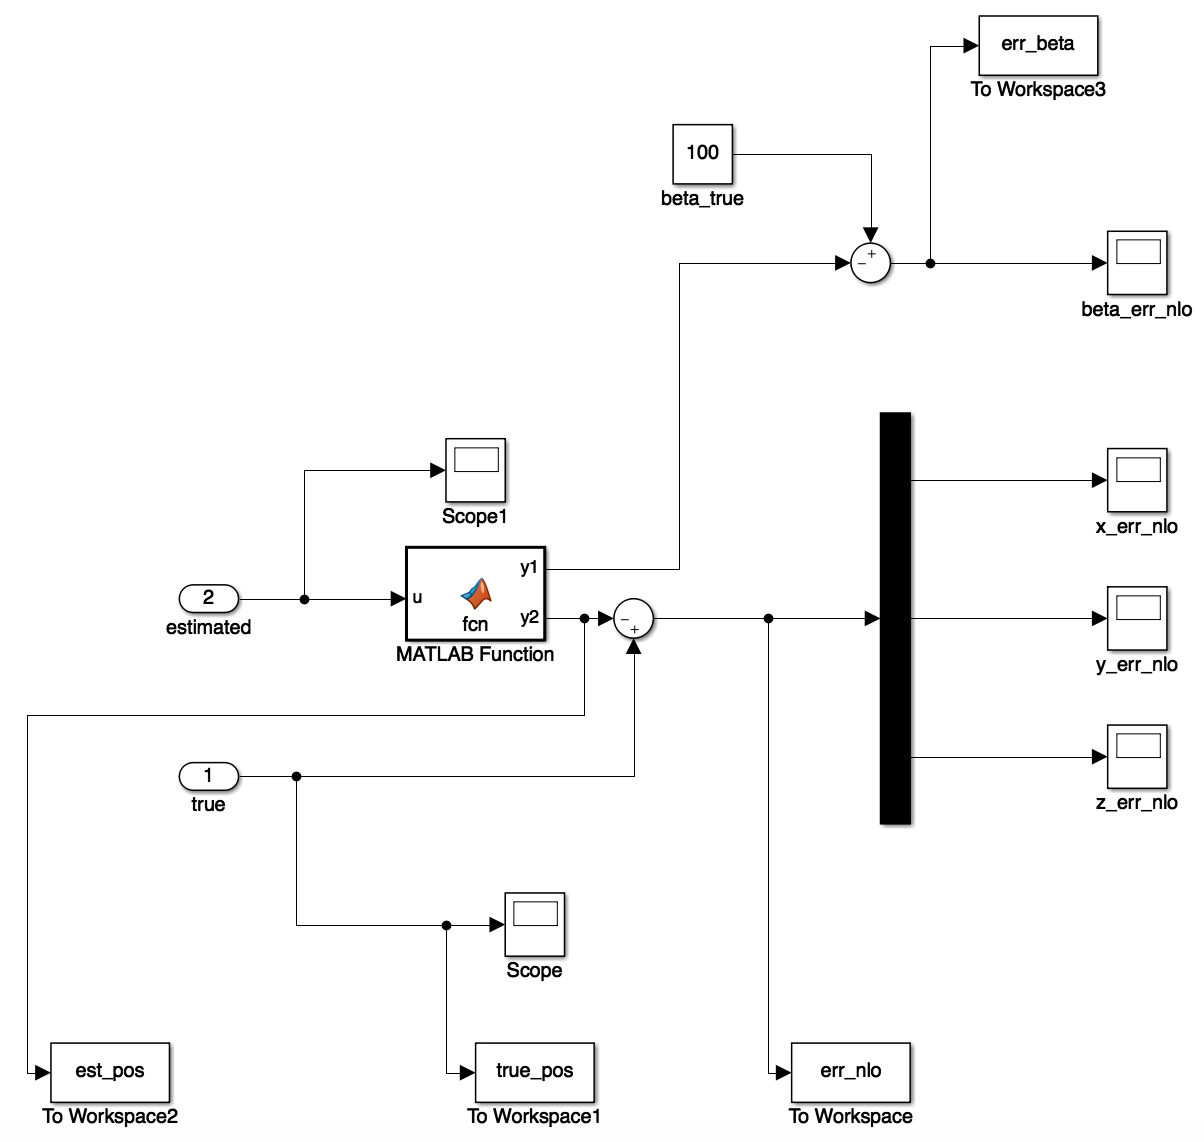
\includegraphics[angle=90,scale = 0.5]{plot_error_TMO.png}
    \caption{Error TMO plots block.}
    \label{fig:f7}
\end{figure}



\begin{figure}
    \centering
    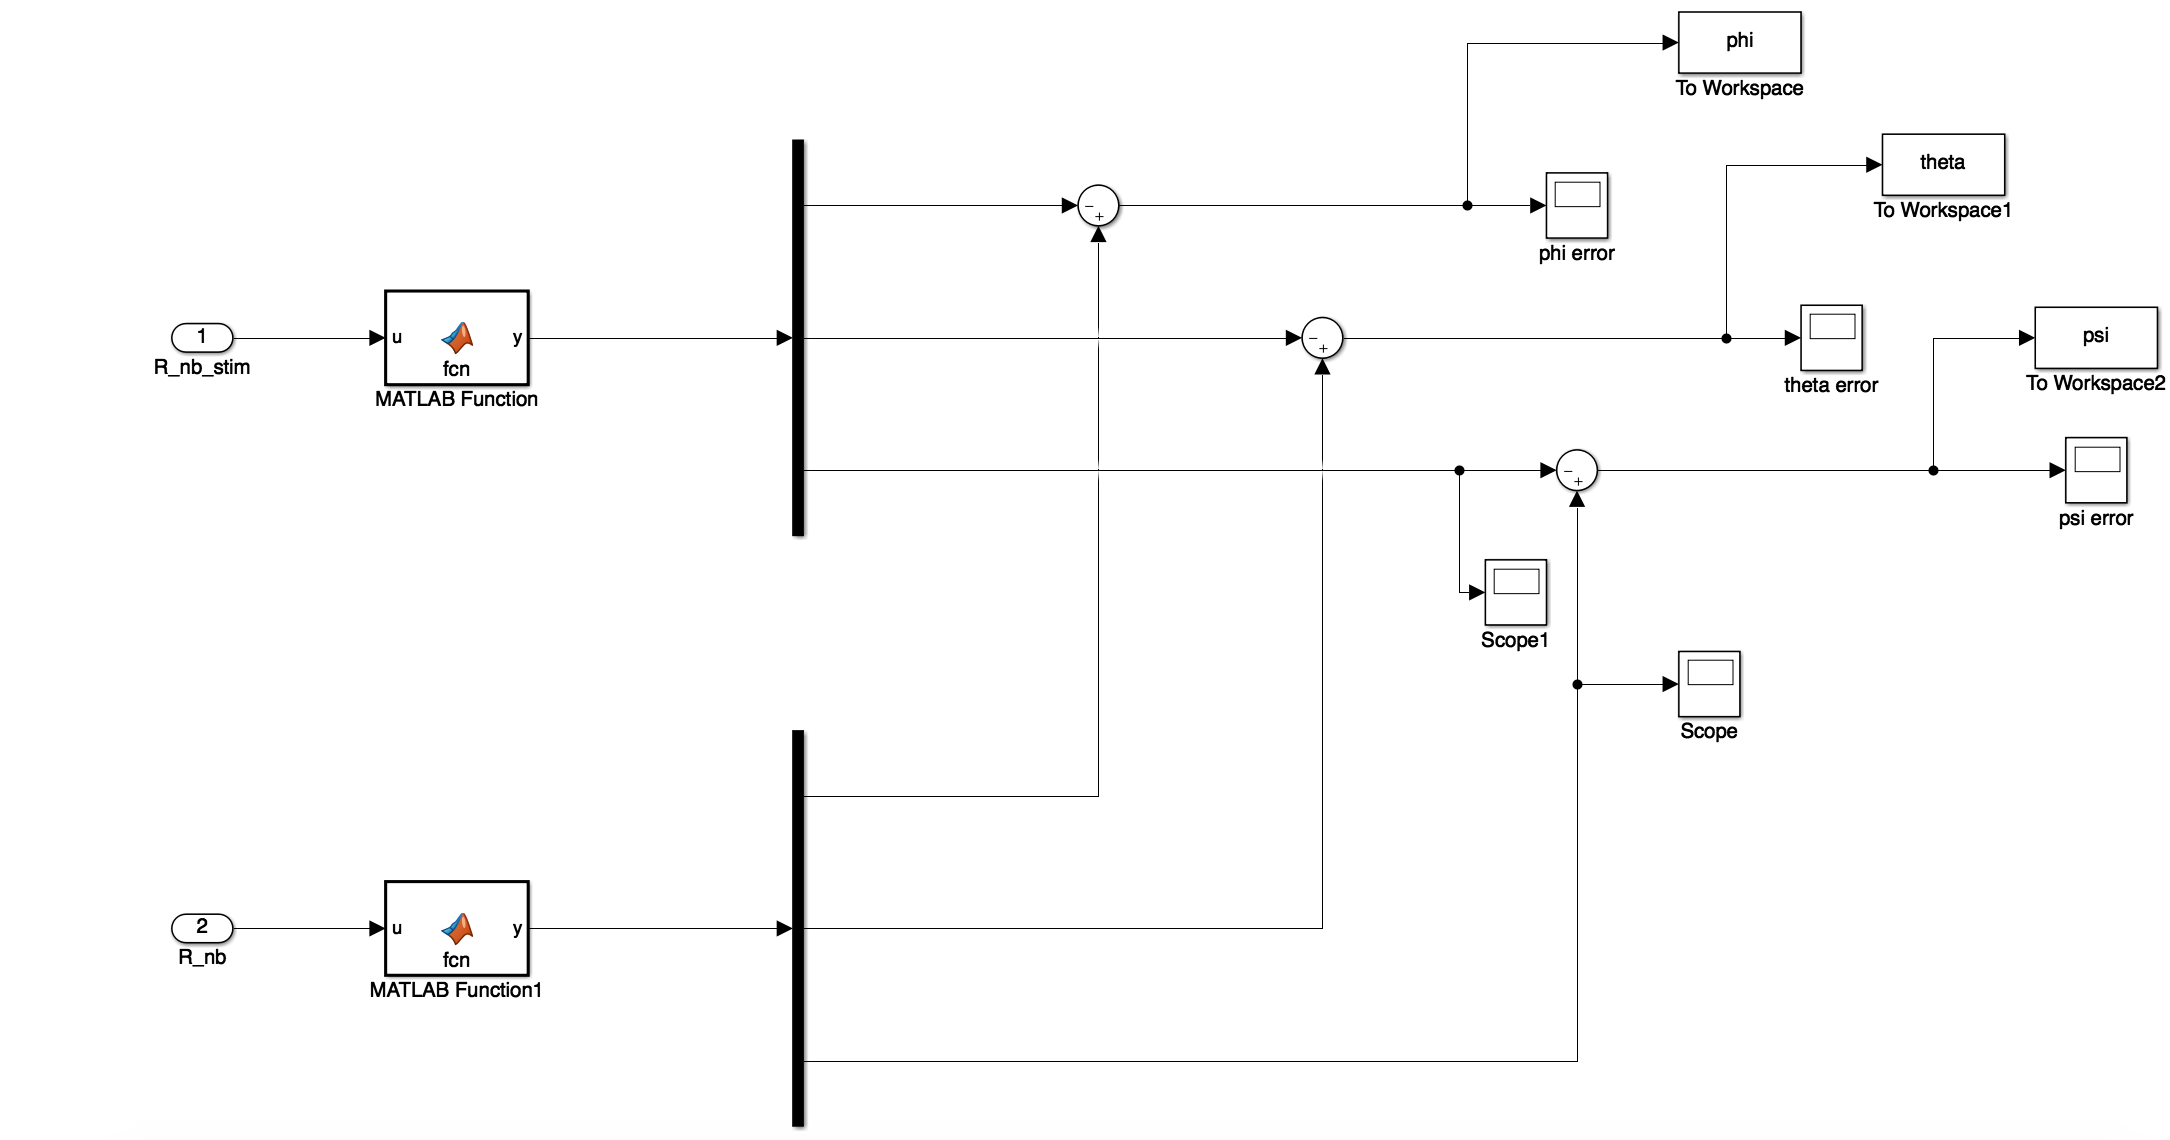
\includegraphics[angle=90,scale = 0.5]{plot_error_mechanization.png}
    \caption{Error mechanization plots block.}
    \label{fig:f8}
\end{figure}



\end{document}
